\section{Goals of the application}
From the analysis of client's needs for the software to be we can derive the following list of goals.
\subsection{Goals Passenger side}
A Passenger:
\begin{enumerate}[label=G.P.{\arabic*})]
\item must be able to register to the service
\item must be able to login to the service
\item can access \textit{myTaxyService} either from the web application or the mobile application
\item must be able to request a taxi ride from a location he decides
\item must be able to reserve a taxi ride from an origin, to a destination at a specific time and date
\item must be able to cancel a reservation that he made
\item must receive, if a taxi is available for a request, a notification stating the arrival time and the taxi identification number
\item if he has reserved a taxi correctly for a certain meeting time, he must be notified before that time with a notification saying the arrival time of the taxi and it identification number, or, in case of problems, saying the nature of the problem.
\end{enumerate}
\subsection{Goals Taxi Driver side}
A Taxi Driver:
\begin{enumerate}[label=G.T.{\arabic*})]
\item must be able to set himself as available (start working) 
\item must be able to set himself as not available (stop working)
\item must receive requests (both immediate and reservations) only if he is available 
\item must be able to choose if he wants to accept an incoming request or not
\item must receive a notification if he is the first taxi in the queue corresponding to his actual location and if a passenger made an request in that zone
\item when available, must be set in the correct waiting queue
\item must receive the location of the passenger who made the request, if he accepted it
\end{enumerate}

\section{Derived behavior of the actors}
From the domain analysis, the assumptions and the basic requirements for the application we can derive a model of behavior of the agents (Passengers and Taxi Drivers) when they use the future application
\subsection{Passenger behavior}
\begin{figure}[H]
\centering
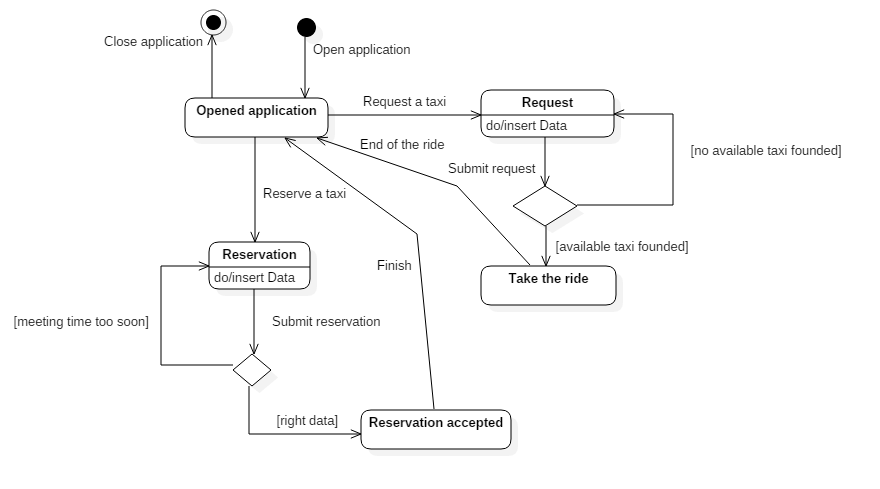
\includegraphics[scale=0.5]{Images/statechart_passenger}
\end{figure}
\subsection{Taxi Driver behavior}
\begin{figure}[H]
\centering
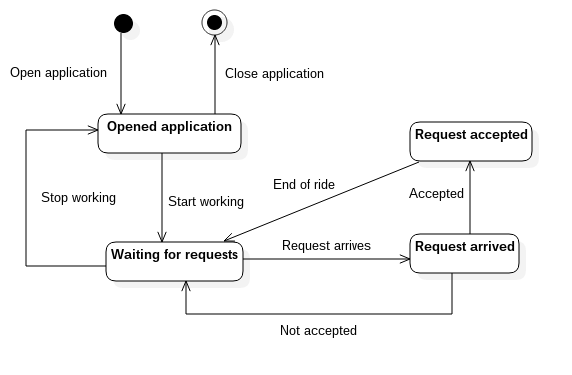
\includegraphics[scale=0.5]{Images/statechart_taxiDriver}
\end{figure}